\documentclass[12pt,a4paper]{article}

\usepackage{graphicx} % For including images
\usepackage{amsmath} % For mathematical equations
\usepackage{amssymb} % For mathematical symbols
\usepackage{float} % To manage figure positioning
\usepackage{geometry} % For page layout
\usepackage[hidelinks]{hyperref} % For hyperlinks
\usepackage{caption} % For customizing figure captions


% Page geometry
\geometry{margin=0.7in}

% Title
\title{Vibrational Analysis with a Focus on Phase-Plane Diagrams}
\author{[Your Name]}
\date{\today}

\begin{document}

% Title Page
\maketitle
\tableofcontents
\newpage

\section{Part 1: Harmonic Force on the Rocket}
\subsection{System Sketch and Representation}
\begin{figure}[H]
    \centering
    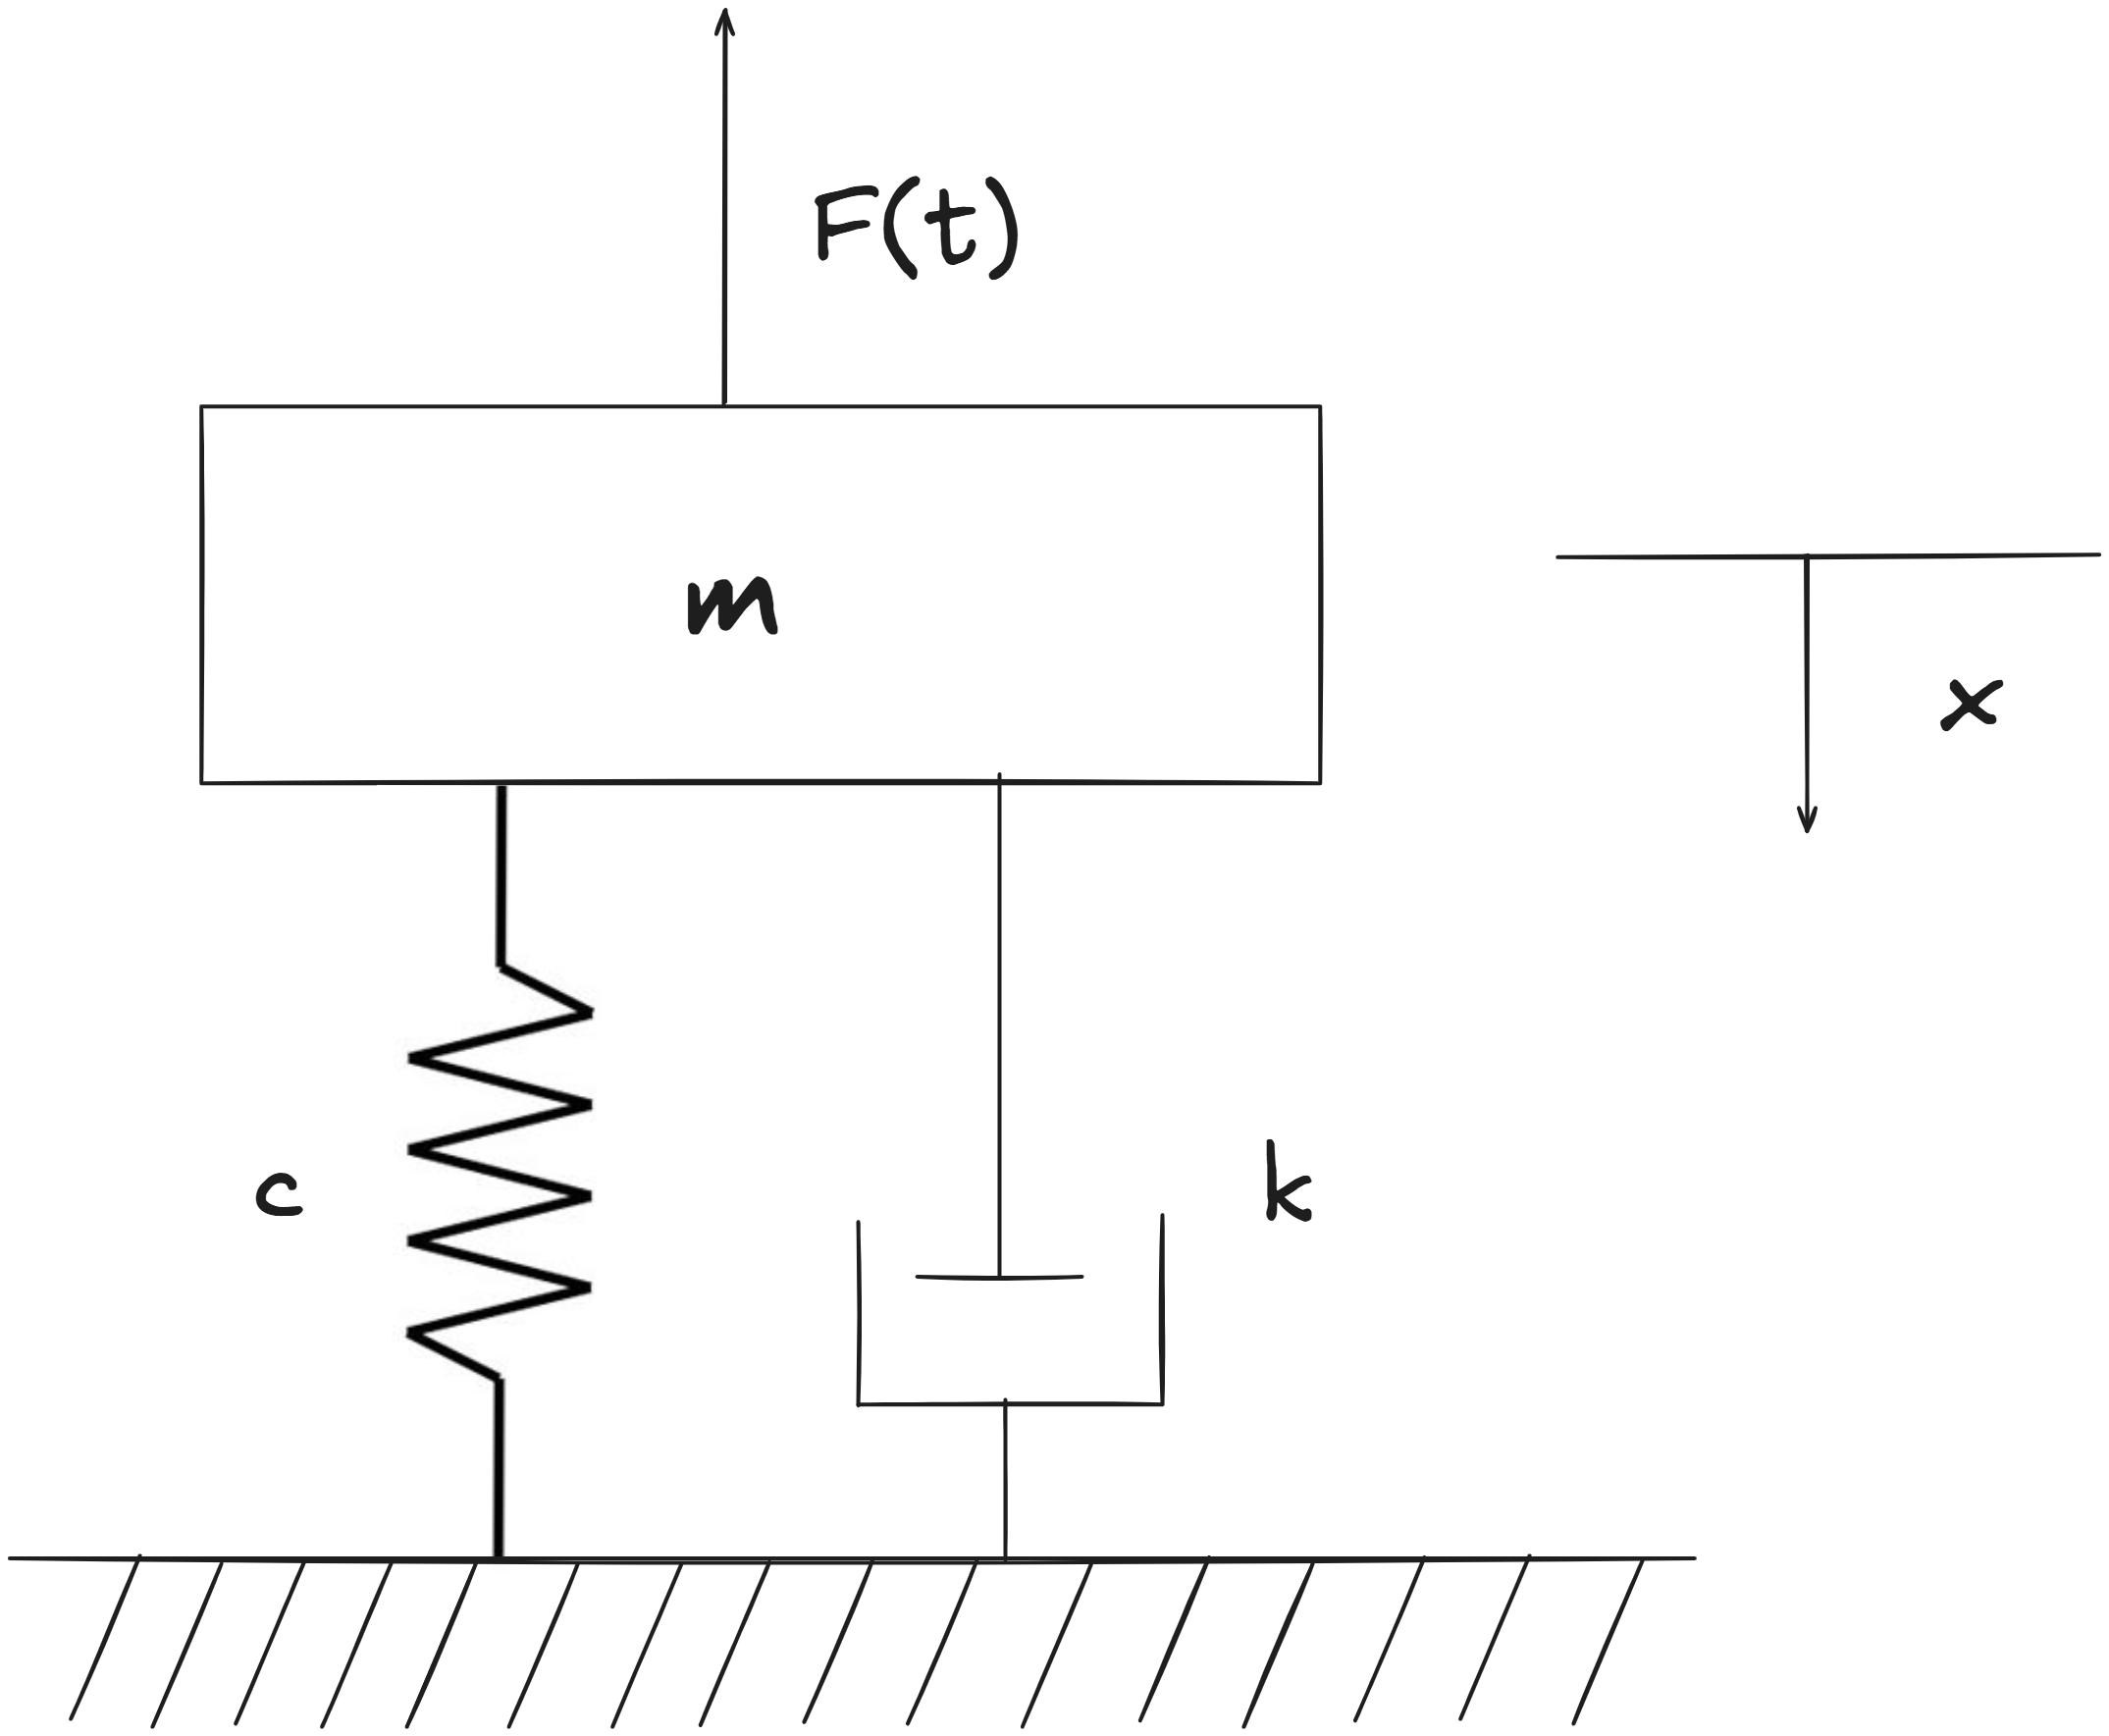
\includegraphics[width=0.8\textwidth]{msd_harmonic.png} 
    \caption{Mass-Spring-Damper System.}
    \label{fig:system}
\end{figure}
\textbf{Where:}
\begin{itemize}
    \item Spring constant, \(c = 20 \, \text{N/m}\)
    \item Damping constant, \(k = 5 \, \text{Ns/m}\)
    \item Mass, \(m = 5 \, \text{kg}\)
    \item Initial position, \(x = 10 \, \text{m}\)
    \item Harmonic Force, \(F(t) = F_0 \cos(\omega t)\)
    \item Angular frequencies, \(\omega = [3, 162, 4.5] \, \text{rad/s}\)
\end{itemize}

\subsection{Hand-Drawn Gaussian Plane: Force Estimation}

\begin{figure}[H]
    \centering
    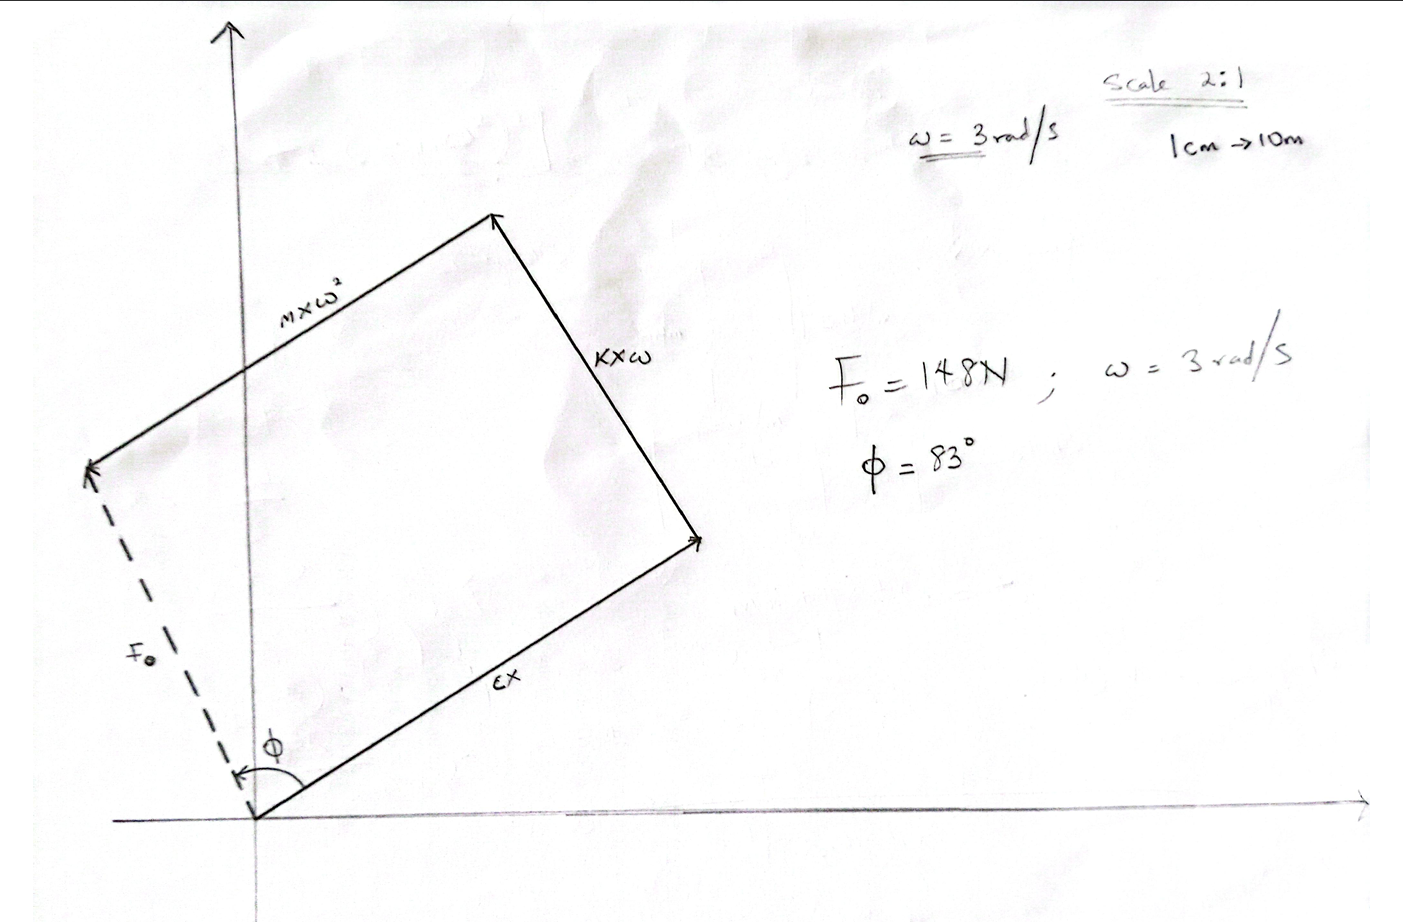
\includegraphics[width=0.8\textwidth]{3rads.png} 
    \caption{Force estimation for $\omega$ = 3 rads/s.}
    \label{fig:system}
\end{figure}

\begin{figure}[H]
    \centering
    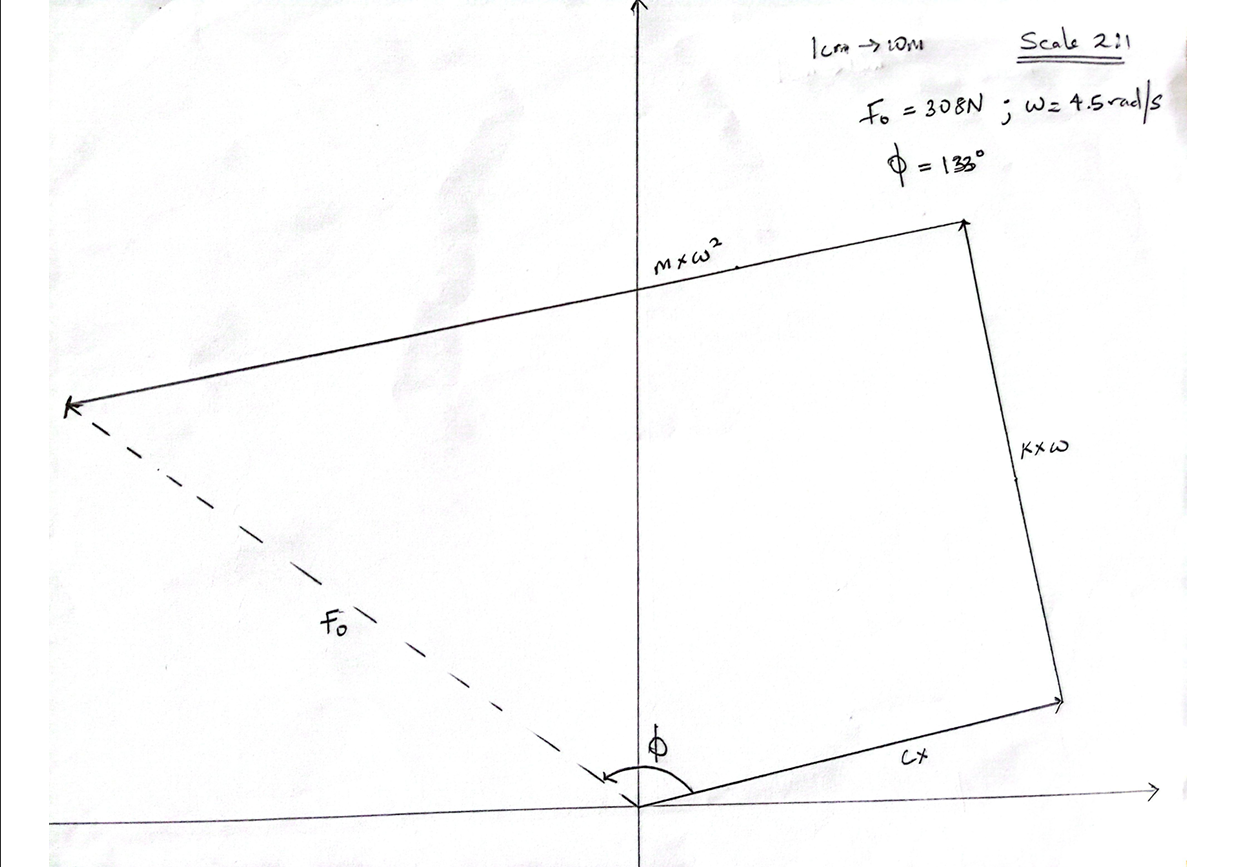
\includegraphics[width=0.8\textwidth]{4.5rads.png} 
    \caption{Force estimation for $\omega$ = 4.5 rads/s.}
    \label{fig:system}
\end{figure}

\begin{figure}[H]
    \centering
    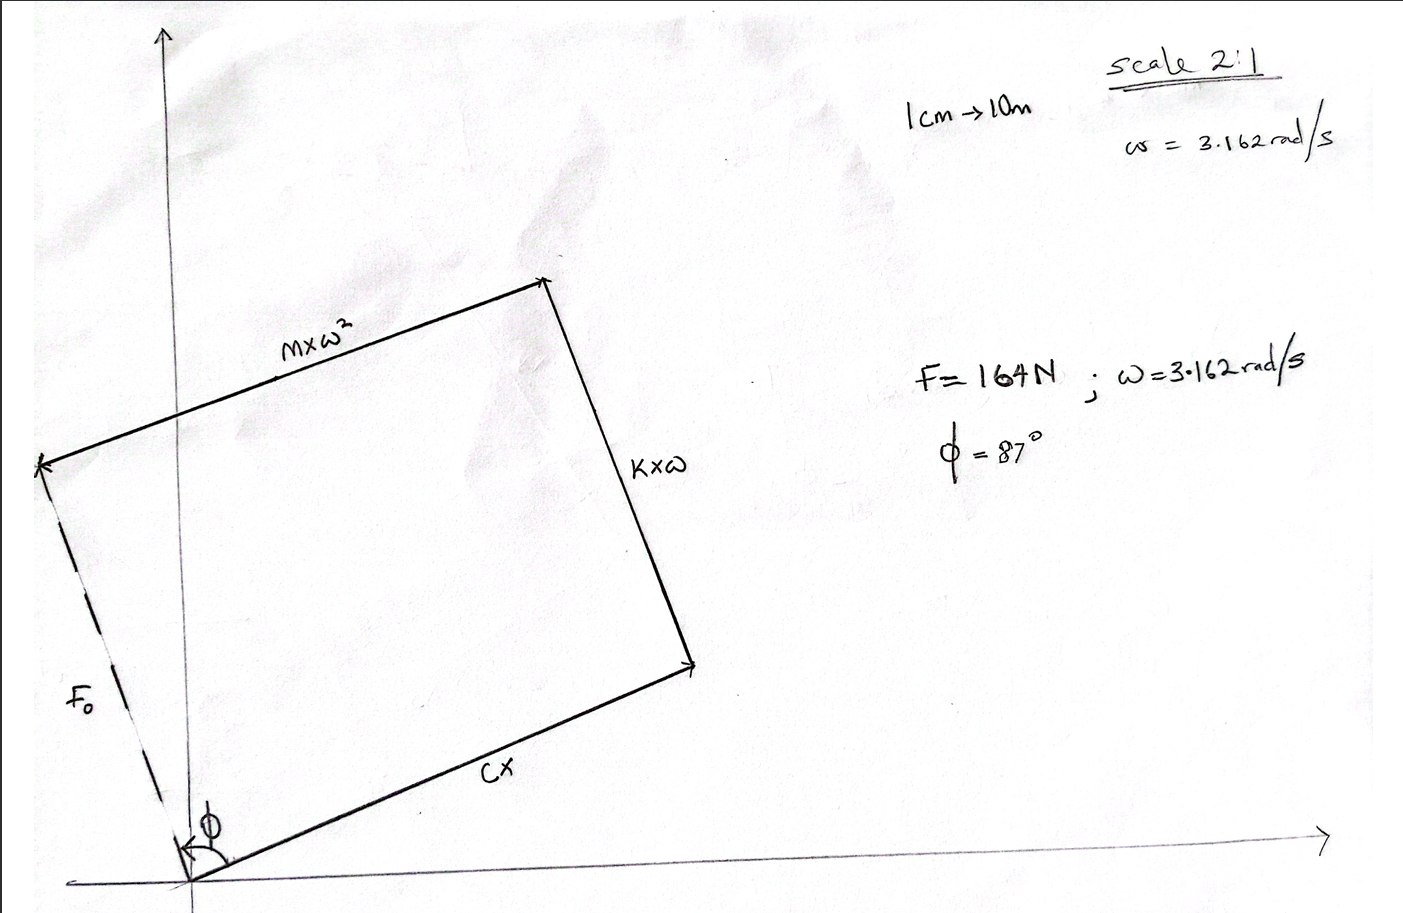
\includegraphics[width=0.8\textwidth]{3.162rads.png} 
    \caption{Force estimation for $\omega$ = 3.162 rads/s.}
    \label{fig:system}
\end{figure}

Disscusion ... 

\subsection{Mathematical Comparison of Forces}

Parameters:
\begin{itemize}
    \item Spring constant, \(c = 20 \, \text{N/m}\)
    \item Damping constant, \(k = 5 \, \text{Ns/m}\)
    \item Mass, \(m = 2 \, \text{kg}\)
    \item Initial position, \(x = 10 \, \text{m}\)
    \item Angular frequencies, \(\omega = [3, 162, 4.5] \, \text{rad/s}\)
\end{itemize}

\noindent\textbf{Amplitude:} 
\[
\hat{X} = \frac{F_{\text{exc}}}{\sqrt{(k \cdot \omega)^2 + (c - m \cdot \omega^2)^2}}
\]

\noindent\textbf{Phase Angle:}
\[
\phi = \tan^{-1} \left( \frac{k \cdot \omega}{c - m \cdot (\omega^2)} \right)
\]

\noindent\textbf{After substituting:}
\begin{itemize}
    \item \(\omega\) = 3 rad/s ; F = 151.33N
    \item \(\omega\) = 3.162 rad/s ; F = 158.1N
    \item \(\omega\) = 4.5 rad/s ; F = 304.38N
\end{itemize}

Compare results from the calculation to that of the hand-drawn approach ...

\subsection{Discussion of the Gaussian Plane Approach}
Reflect on how well the graphical estimation matches the mathematical computation ...
{\vspace{5pt}}
Discuss the usefulness of the Gaussian plane method in understanding force relationships ... 

\subsection{Damping Ratio and Curl}
\begin{figure}[H]
    \centering
    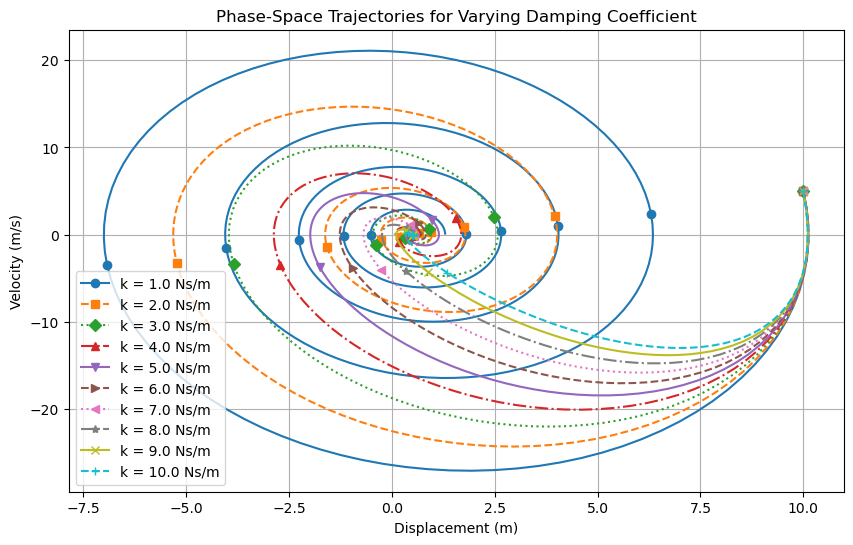
\includegraphics[width=0.8\textwidth]{damping_ratio_to_curl.png} 
    \caption{Phase Trajectory for Varying Damping Coefficient}
    \label{fig:system}
\end{figure}
{\vspace{10pt}}
Discussion
{\vspace{10pt}}

\subsection{Angular Frequency and Its Effect on the System}
\begin{figure}[H]
    \centering
    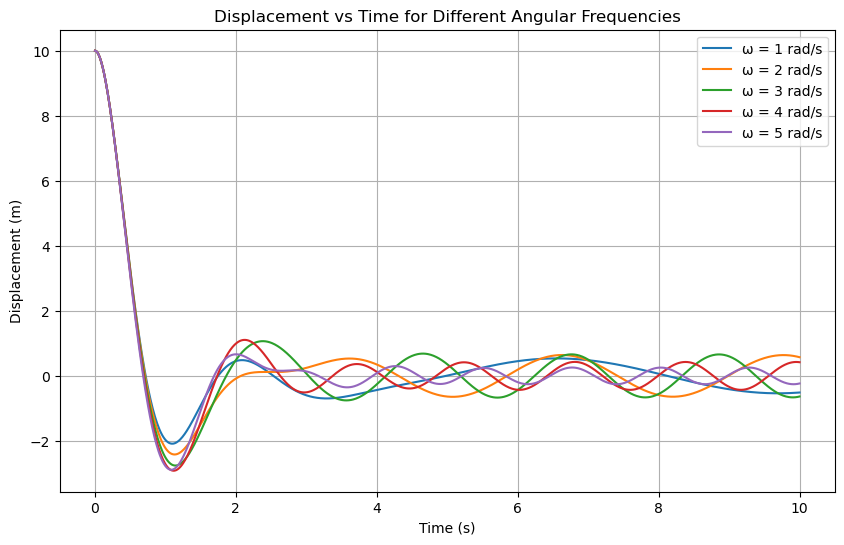
\includegraphics[width=0.8\textwidth]{angular_freq_effect_on_system.png} 
    \caption{Displacement vs Time for Different Angular Frequencies}
    \label{fig:system}
\end{figure}
{\vspace{10pt}}
Discussion
{\vspace{10pt}}

\subsection{Varying the Spring Constant}
\begin{figure}[H]
    \centering
    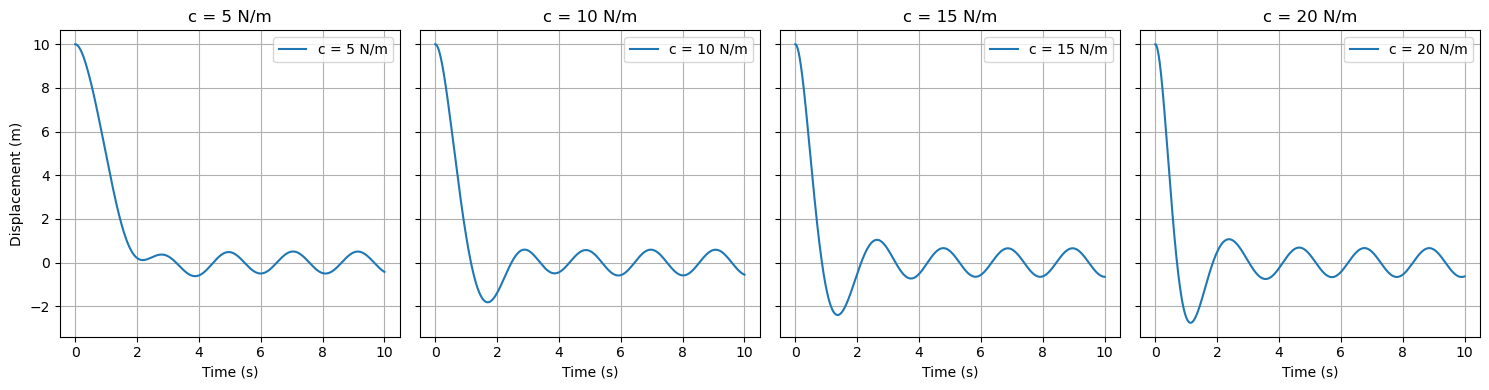
\includegraphics[width=0.8\textwidth]{spring_constant_effect_on_system.png} 
    \caption{Displacement vs Time for Different Angular Frequencies}
    \label{fig:system}
\end{figure}
{\vspace{10pt}}
Discussion
{\vspace{10pt}}


\subsection{Square Wave Analysis}
\subsubsection{System Responses}
\begin{figure}[H]
    \centering
    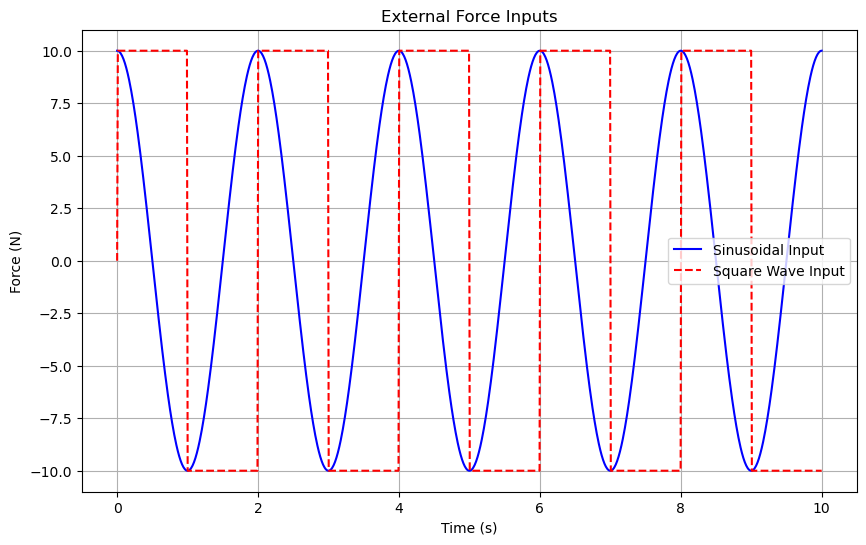
\includegraphics[width=0.8\textwidth]{force_input.png} 
    \caption{External Force Input}
    \label{fig:system}
\end{figure}
{\vspace{10pt}}
Discussion
{\vspace{10pt}}

\begin{figure}[H]
    \centering
    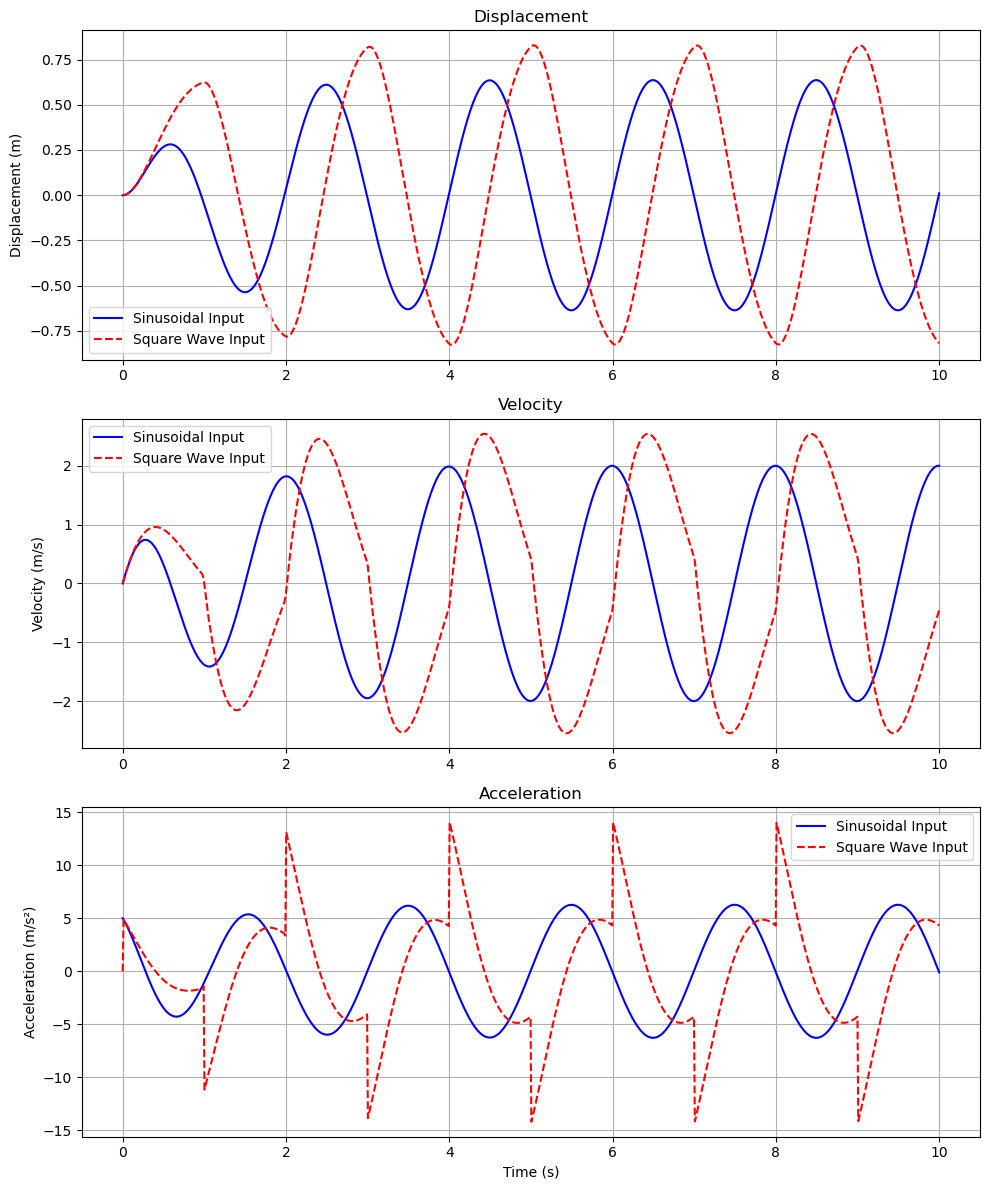
\includegraphics[width=0.8\textwidth]{disp_vel_acc.png  } 
    \caption{Displacement, Velocity and Acceleration }
    \label{fig:system}
\end{figure}
{\vspace{10pt}}
Discussion
{\vspace{10pt}}

\subsubsection{Frequency Domain Analysis}
\begin{figure}[H]
    \centering
    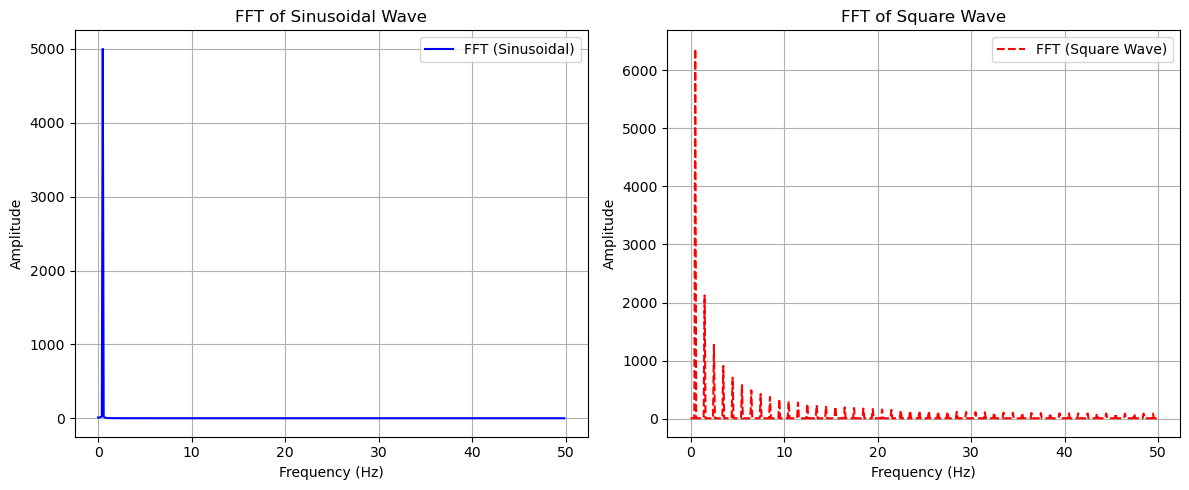
\includegraphics[width=0.8\textwidth]{freq_domain.png} 
    \caption{Frequency Domain Analysis}
    \label{fig:system}
\end{figure}
{\vspace{10pt}}
Discussion
{\vspace{10pt}}

\section{Part 2: Base Motion in the Rocket}

\subsection{System Sketch and Representation}
\begin{figure}[H]
    \centering
    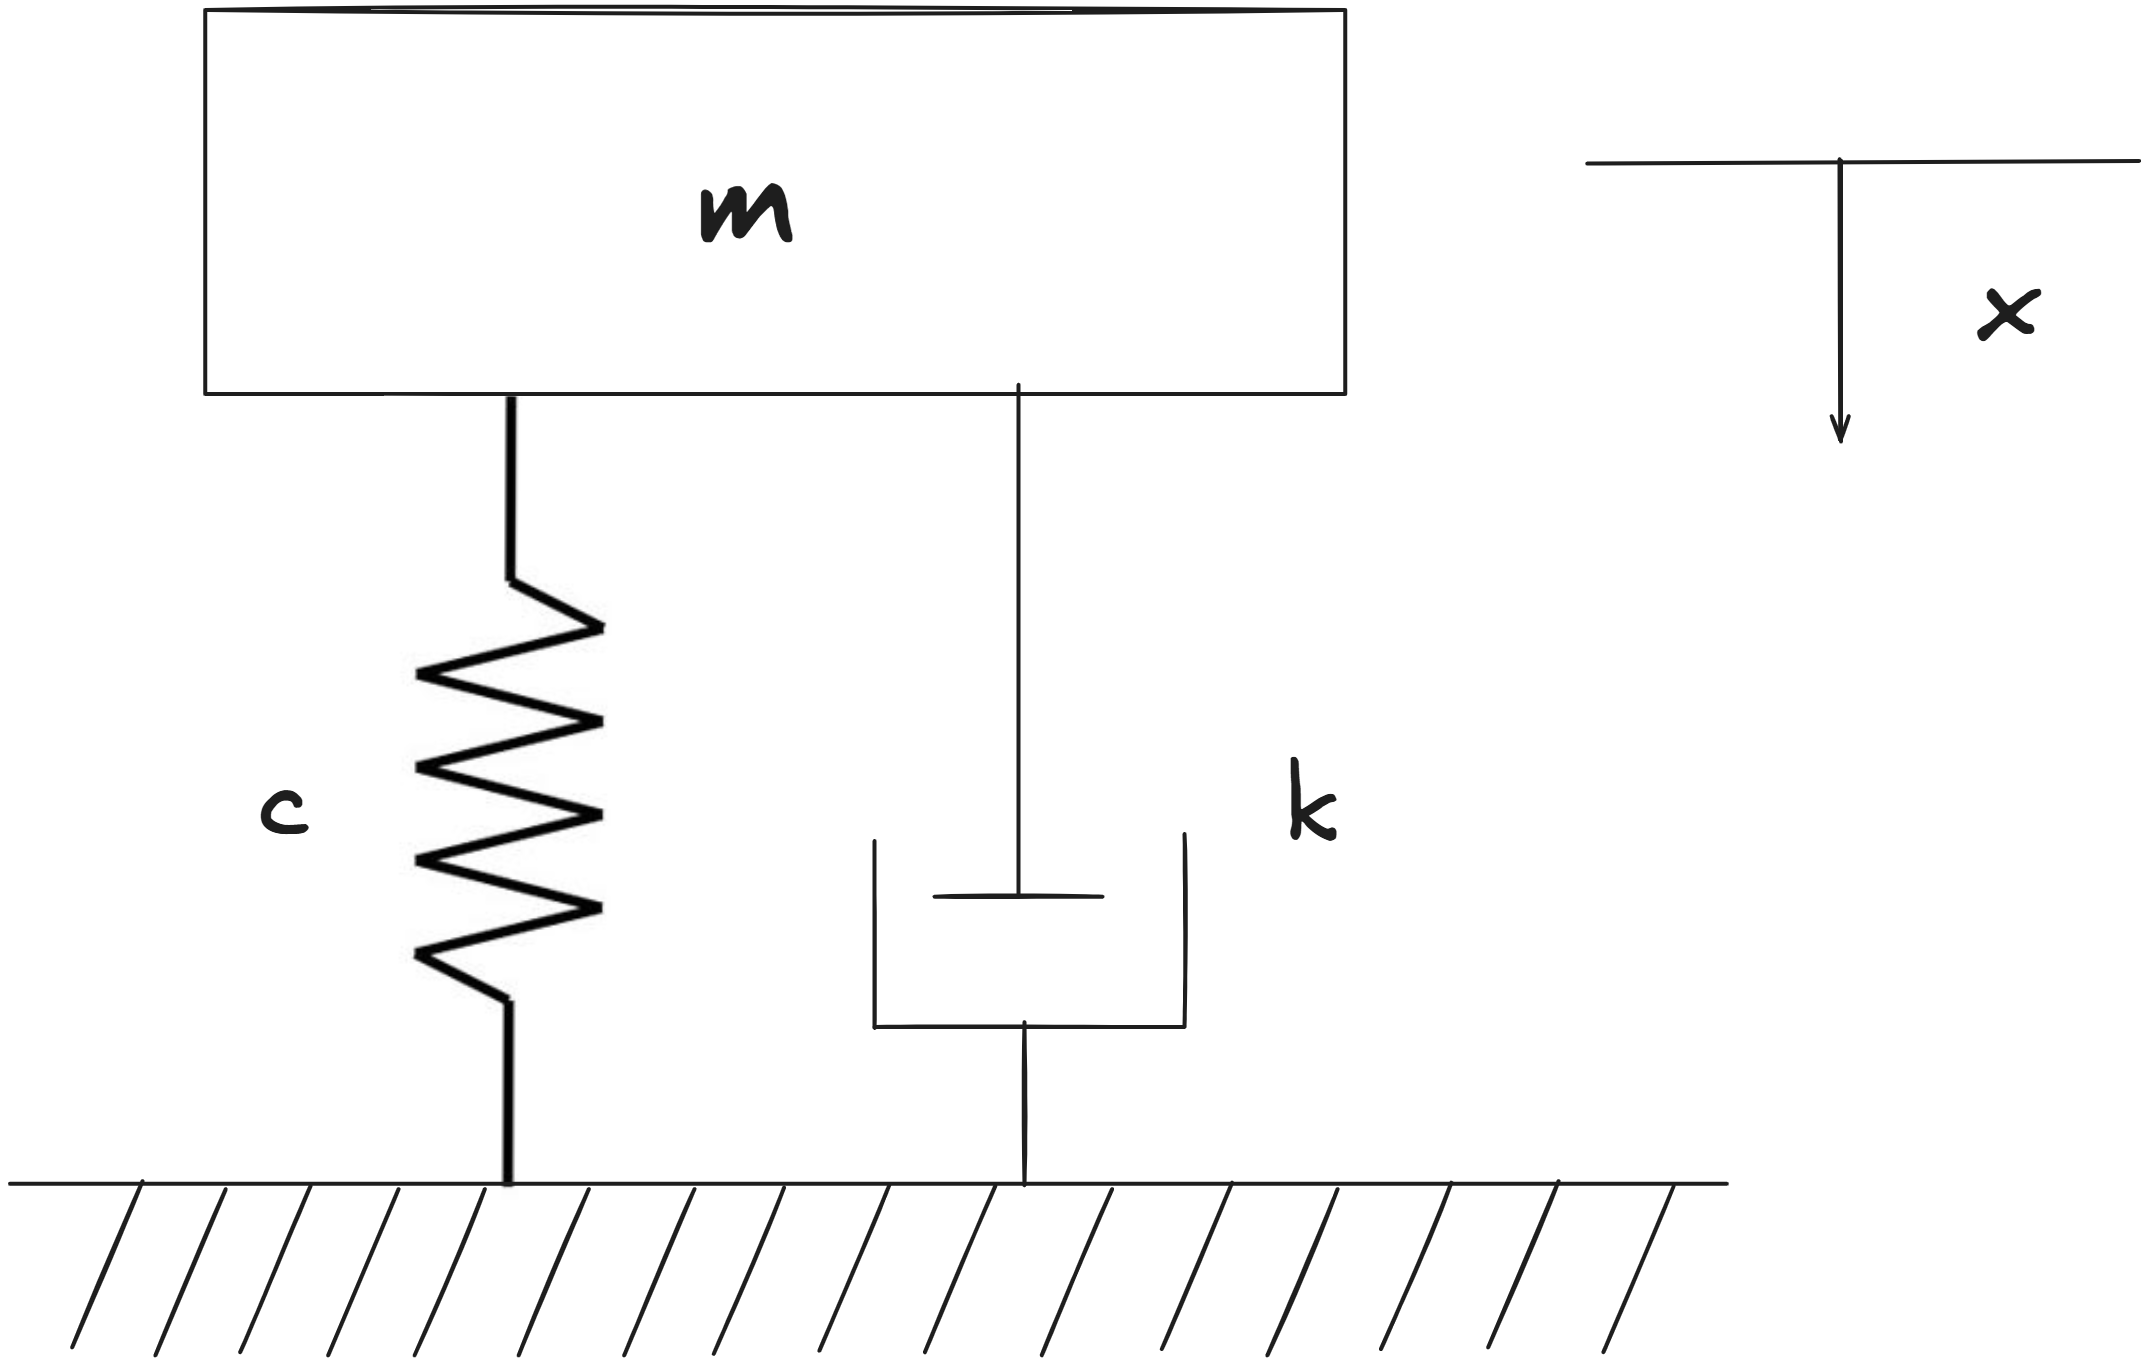
\includegraphics[width=0.8\textwidth]{msd.png} 
    \caption{Mass-Spring-Damper System.}
    \label{fig:system}
\end{figure}
\textbf{Where:}
\begin{itemize}
    \item Spring constant, \(c = 20 \, \text{N/m}\)
    \item Damping constant, \(k = 5 \, \text{Ns/m}\)
    \item Mass, \(m = 5 \, \text{kg}\)
    \item Initial position, \(x = 10 \, \text{m}\)
\end{itemize}

\subsection{Damped and Undamped Responses}
\begin{figure}[H]
    \centering
    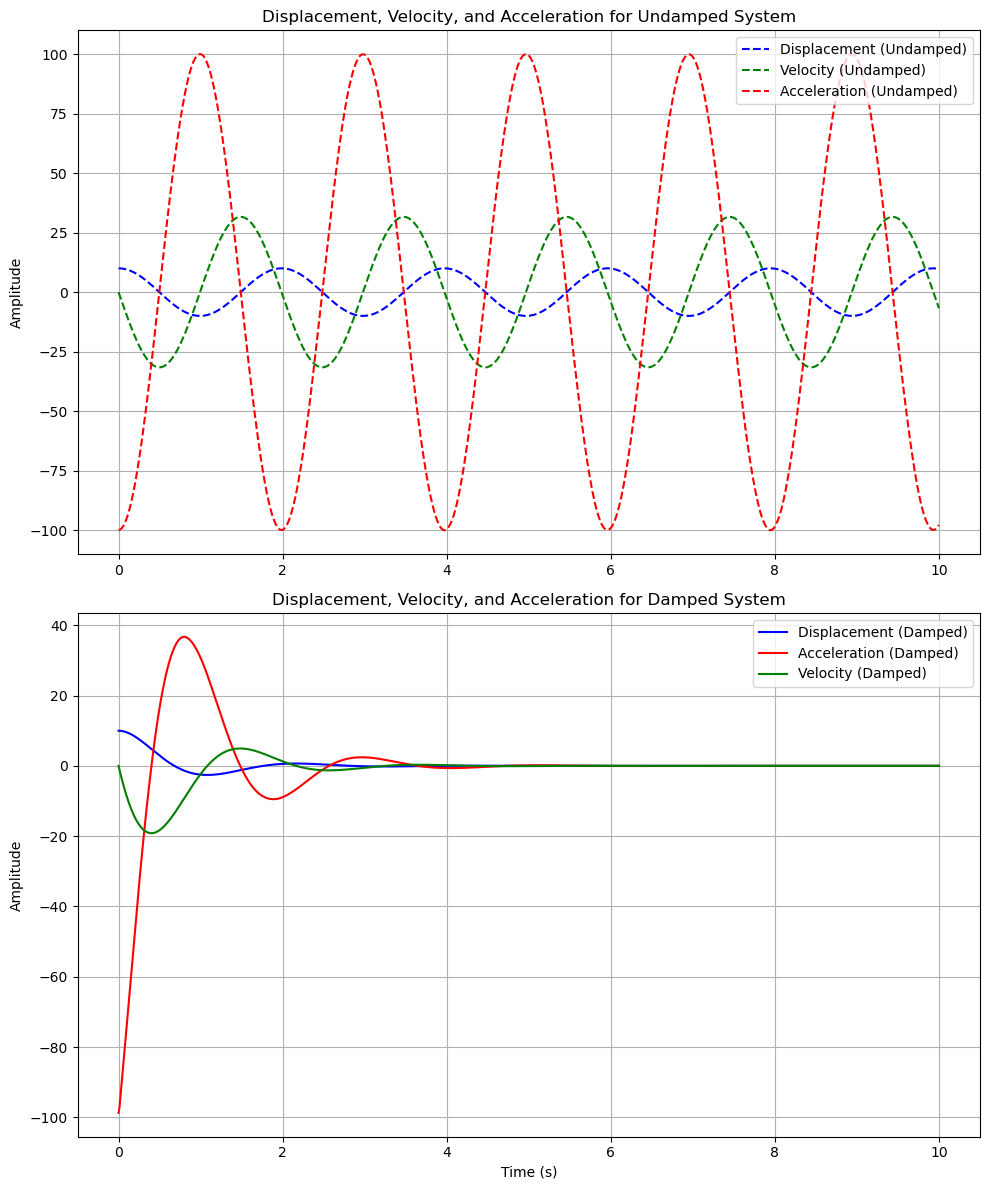
\includegraphics[width=0.8\textwidth]{disp_vel_acc_damp_and_undamp.png} 
    \caption{Displacement, Velocity and acceleration for Damped and Undamped system.}
    \label{fig:system}
\end{figure}
{\vspace{10pt}}
Discussion
{\vspace{10pt}}


\subsection{Mass Spring Damper with moving Base}
\begin{figure}[H]
    \centering
    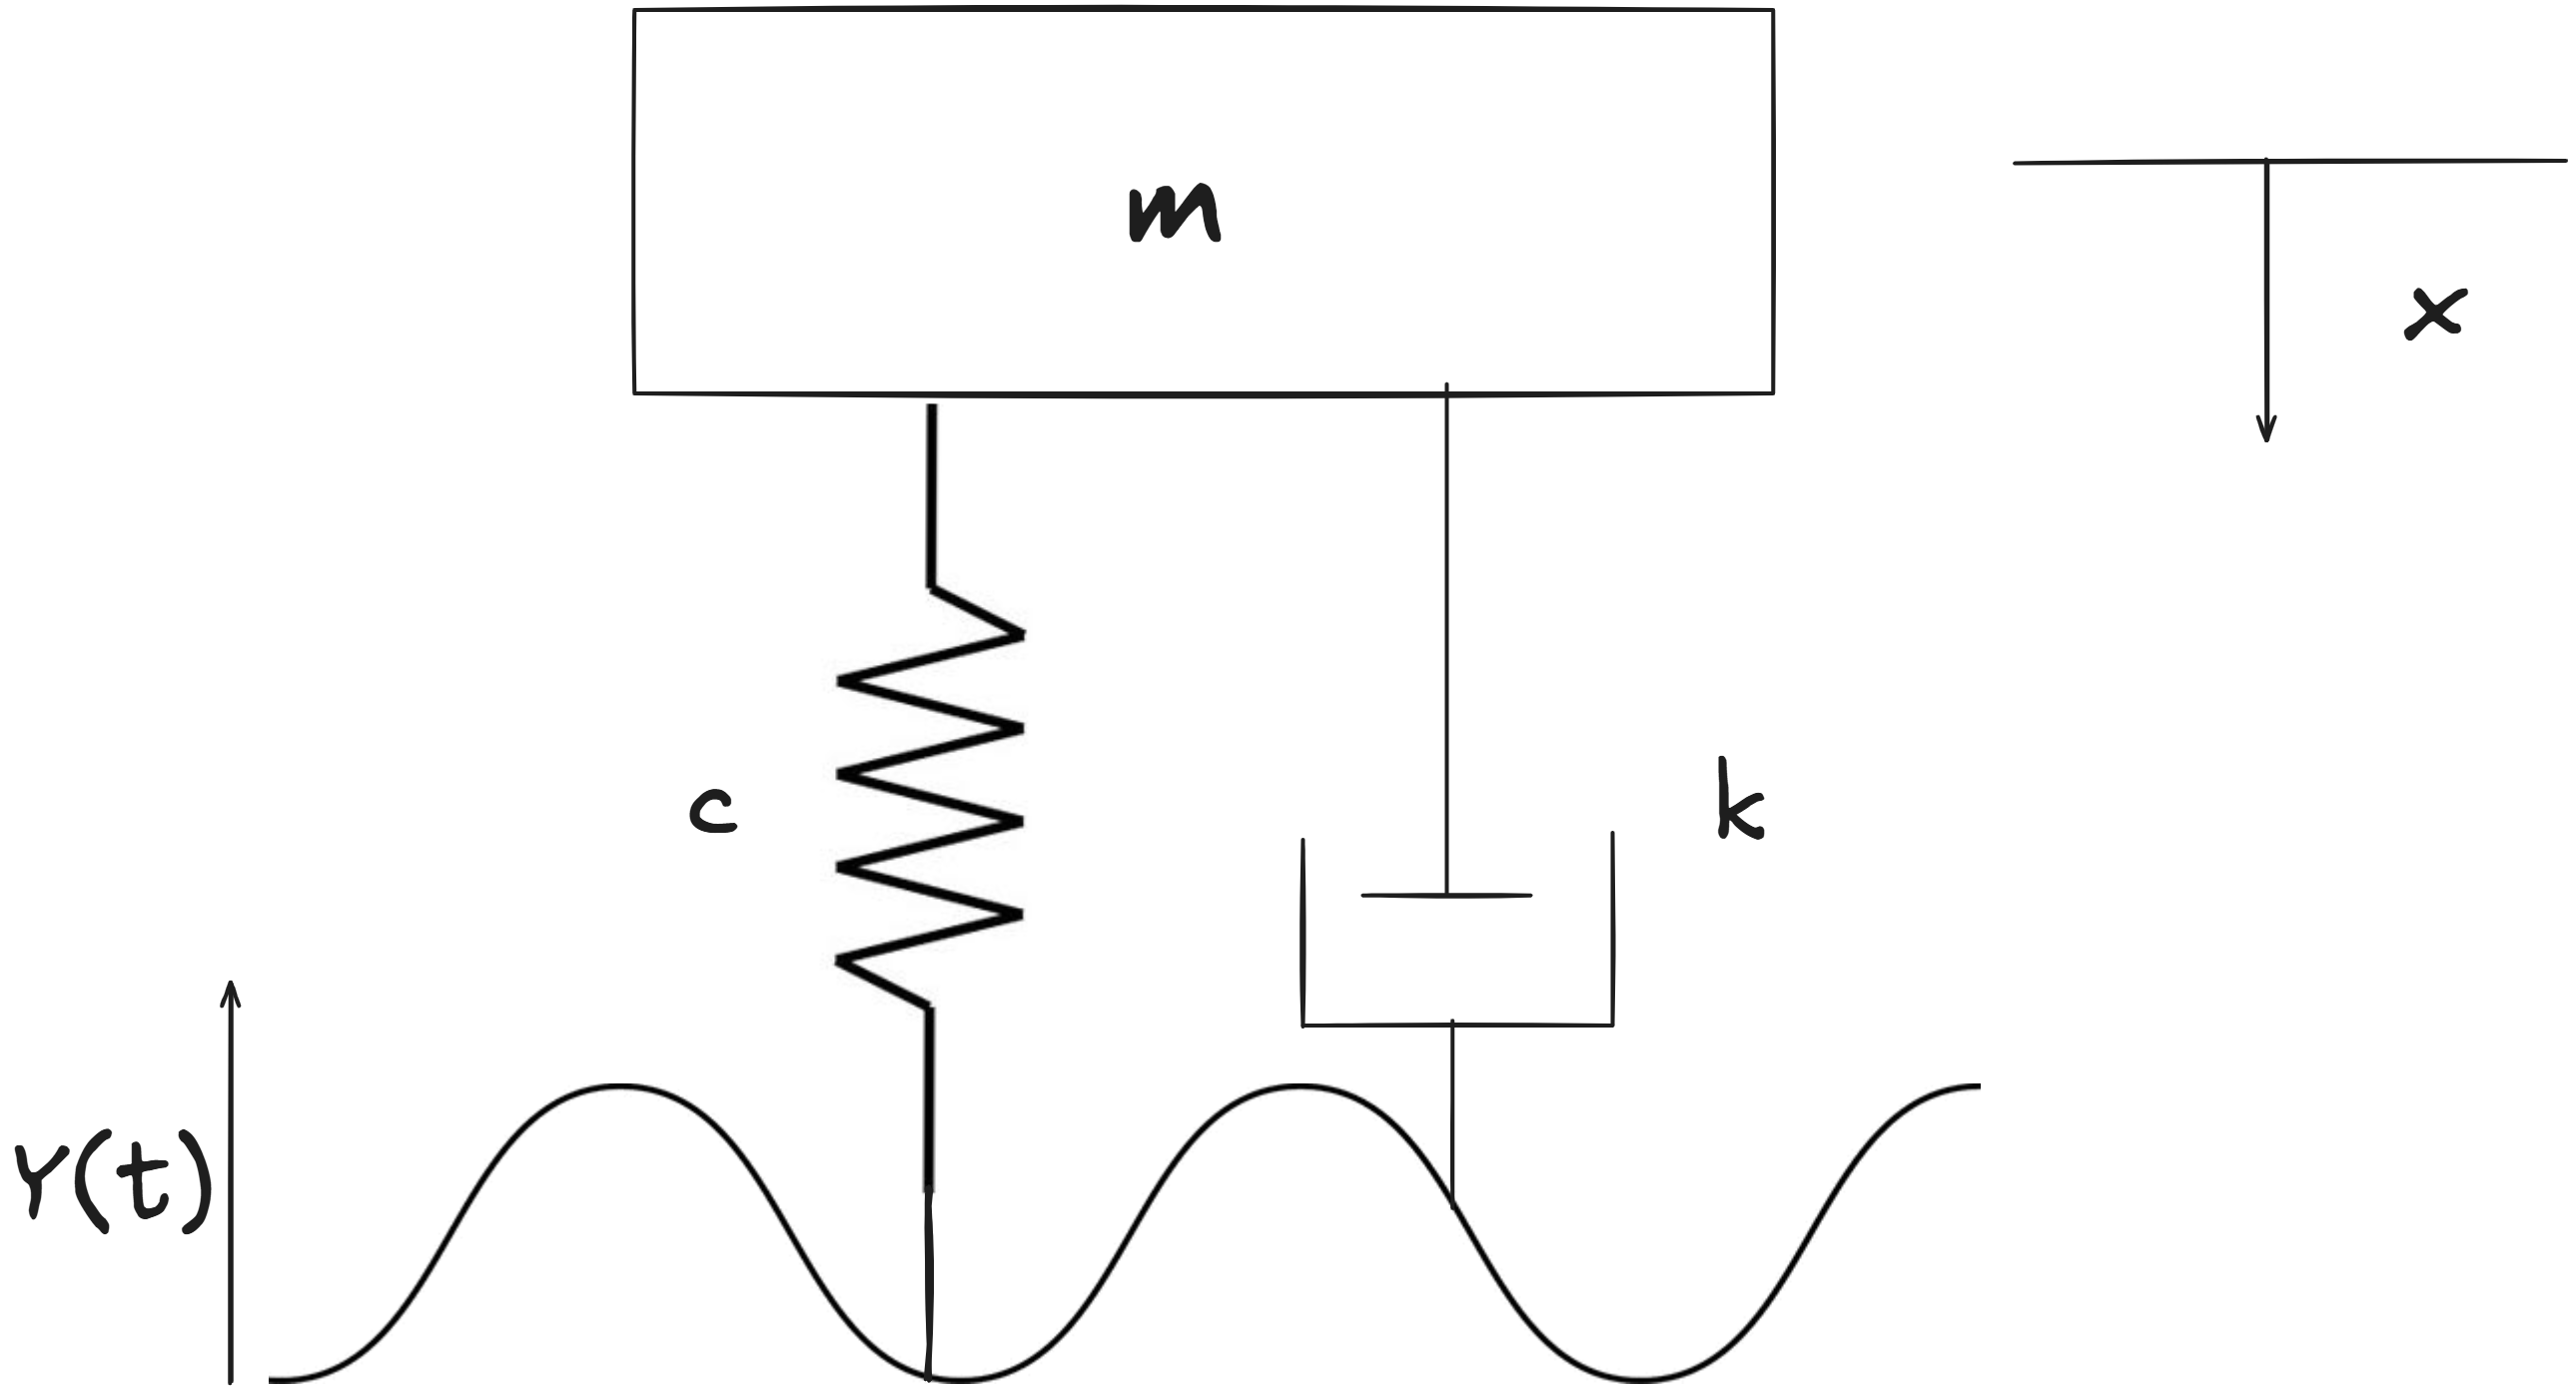
\includegraphics[width=0.8\textwidth]{msd_base.png} 
    \caption{Mass-Spring-Damper system with moving base.}
    \label{fig:system}
\end{figure}
\textbf{Where:}
\begin{itemize}
    \item Mass, \(m = 5 \, \text{kg}\)
    \item Spring constant, \(c = 20 \, \text{N/m}\)
    \item Damping constant, \(k = 5 \, \text{Ns/m}\)
    \item Initial position, \(x = 10 \, \text{m}\)
    \item Base Force, \(Y(t) = Y_0 \cos(\omega t)\)    
\end{itemize}

\subsection{Amplitude and Phase Angle}

Calculating Amplitude and Phase Angle:  

{\vspace{5pt}}

\textbf{Given:}

- Base Excitation Force: 
\[
Y(t) = Y_0 \cos(\omega t)
\]
\[
\dot{Y}(t) = -\omega Y_0 \sin(\omega t)
\]

- Angular Frequency: 
\[
\omega = \frac{2 \pi}{l}
\]

\textbf{Given:}
\begin{itemize}
    \item \( V = 2000 \, \text{m/s} \)
    \item \( l = 1000 \, \text{m} \)
\end{itemize}

\[
\omega = 12.566 \, \text{rad/s}
\]

The system model is given by:

\[
m \ddot{x}  + k \dot{x} + c x = y(t)
\]

where:
\begin{itemize}
    \item \( m = \text{Mass} \)
    \item \( k = \text{Damping Constant} \)
    \item \( c = \text{Spring Constant} \)
    \item \( x = \text{Displacement} \)
    \item \( \dot{x} = \text{Velocity} \)
    \item \( \ddot{x} = \text{Acceleration} \)
    \item \( Y(t) = Y \cos(\omega t) \)
\end{itemize}

{\vspace{5pt}}

From Newton's Second Law, \( \sum F = ma \), we have:

\[
m \ddot{x} + k (\dot{x} - \dot{Y}) + c(x - Y) = 0
\]
\[
m \ddot{x} + k \dot{x} - k \dot{Y} + c x - cY = 0
\]
\[
m \ddot{x} + k \dot{x} + c x = c Y + k \dot{Y}
\]

{\vspace{5pt}}

Substituting for \( y \) and \( \dot{y} \), we have:

\[
m \ddot{x} + k \dot{x} + c x = c Y \cos(\omega t) - k \omega Y \sin(\omega t)
\]

{\vspace{5pt}}

We know that:

\[
x = X_0 \cos(\omega t - \phi) \quad \text{(eq. 1)}
\]
\[
\dot{x} = -\omega X_0 \sin(\omega t - \phi) \quad \text{(eq. 2)}
\]
\[
\ddot{x} = -\omega^2 X_0 \cos(\omega t - \phi) \quad \text{(eq. 3)}
\]

{\vspace{5pt}}

Substituting eq. (1), eq. (2), and eq. (3) into the system model, we have:

\[
m (-\omega^2 X_0 \cos(\omega t - \phi)) + k (-\omega X_0 \sin(\omega t - \phi)) + c (X_0 \cos(\omega t - \phi)) = c Y \cos(\omega t) - k \omega Y \sin(\omega t)
\]

{\vspace{5pt}}

After Phasor representation, we have:

\[
F_{\text{res1}}^2 = c Y^2 + k Y \omega^2
\]
\[
= Y^2 (c^2 + k^2 \omega^2)
\]

\[
F_{\text{res2}}^2 = (k X_0 \omega)^2 + (c X_0 - m X_0 \omega)^2
\]
\[
= X_0^2 \left[ (k \omega)^2 + (c - m \omega^2)^2 \right]
\]

{\vspace{5pt}}

Equating \( F_{\text{res1}}^2 \) and \( F_{\text{res2}}^2 \), we have:

\[
Y^2 (c^2 + k^2 \omega^2) = X_0^2 \left[ (k \omega)^2 + (c - m \omega^2)^2 \right]
\]

{\vspace{5pt}}

Equations for \( X_0 \) and \( \phi \), we have:

\[
X_0 = Y_0 \sqrt{ \frac{c^2 + (k \omega)^2}{(k \omega)^2 + (c - m \omega^2)^2} }
\]

\[
\phi = \tan^{-1}\left( \frac{m \omega^3 k}{c^2 - m \omega^2 c + k^2 \omega^2} \right)
\]

{\vspace{5pt}}

Solving for \( X_0 \) and \( \phi \):

Given:
\begin{itemize}
    \item \( m = 2 \, \text{kg} \)
    \item \( k = 5 \, \text{N/m} \)
    \item \( c = 20 \, \text{Ns/m} \)
    \item \( Y_0 = 150 \, \text{m} \)
    \item \( \omega = 12.566 \, \text{rad/s} \)
\end{itemize}

{\vspace{5pt}}

We have:

\[
X_0 = 151 \sqrt{ \frac{20^2 + (5 \times 12.566)^2}{(5 \times 12.566)^2 + (20 - 2 \times (12.566)^2)^2} }
\]

\[
\phi = \tan^{-1}\left( \frac{2 \times (12.566)^3 \times 5}{20^2 - 2 \times (12.566)^2 \times 20 + 5^2 \times (12.566)^2} \right)
\]

{\vspace{5pt}}

Thus:

\[
X_0 = 32.92 \, \text{m}
\]
\[
\phi = -84.334 \, \text{rad/s} \quad (95.67^\circ)
\]

{\vspace{5pt}}

\subsection{State Space Representation}
State-Space Representation:
\[
\dot{X} = \underset{\rightarrow}{A}\vec{x} + \underset{\rightarrow}{B}\vec{y}
\]

Introduce the state variables:
\[
x_1 = x, \quad x_2 = \dot{x}
\]

This gives:
\[
\dot{x}_1 = x_2, \quad \dot{x}_2 = \ddot{x}
\]

From the differential equation:
\[
m\ddot{x} = -k\dot{x} - cx + k\dot{Y} + cY
\]

Re-arranging for \( \ddot{x} \):
\[
\dot{x}_2 = -\frac{c}{m}x_1 - \frac{k}{m}x_2 + \frac{k}{m}\dot{Y} + \frac{c}{m}Y
\]

Now, the state-space form becomes:
\[
\begin{bmatrix}
\dot{x}_1 \\
\dot{x}_2
\end{bmatrix}
=
\underbrace{
\begin{bmatrix}
0 & 1 \\
-\frac{c}{m} & -\frac{k}{m}
\end{bmatrix}}_{A}
\begin{bmatrix}
x_1 \\
x_2
\end{bmatrix}
+
\underbrace{
\begin{bmatrix}
0 & 0 \\
\frac{c}{m} & \frac{k}{m}
\end{bmatrix}}_{B}
\begin{bmatrix}
Y \\
\dot{Y}
\end{bmatrix}
\]

Here:
\begin{itemize}
    \item \( A \) is the system matrix.
    \item \( B \) accounts for the influence of \( Y(t) \) and \( \dot{Y}(t) \), the base motion and its velocity.
\end{itemize}
   


\subsection{Impact of Base Excitation Amplitude}
\begin{figure}[H]
    \centering
    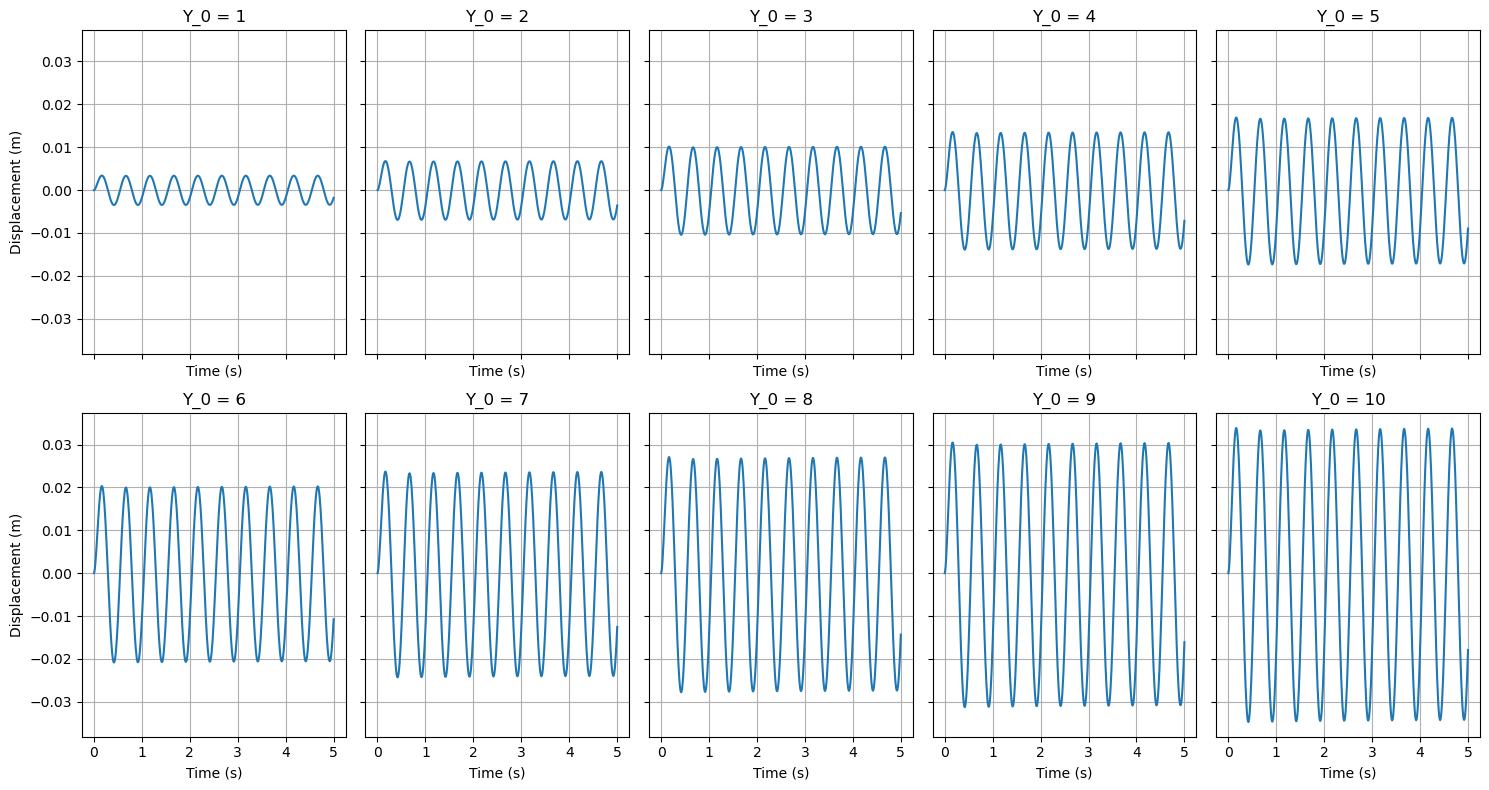
\includegraphics[width=0.8\textwidth]{disp_response.png} 
    \caption{Displacement Response for different Y0 values}
    \label{fig:system}
\end{figure}
{\vspace{10pt}}
Discussion
{\vspace{10pt}}

\begin{figure}[H]
    \centering
    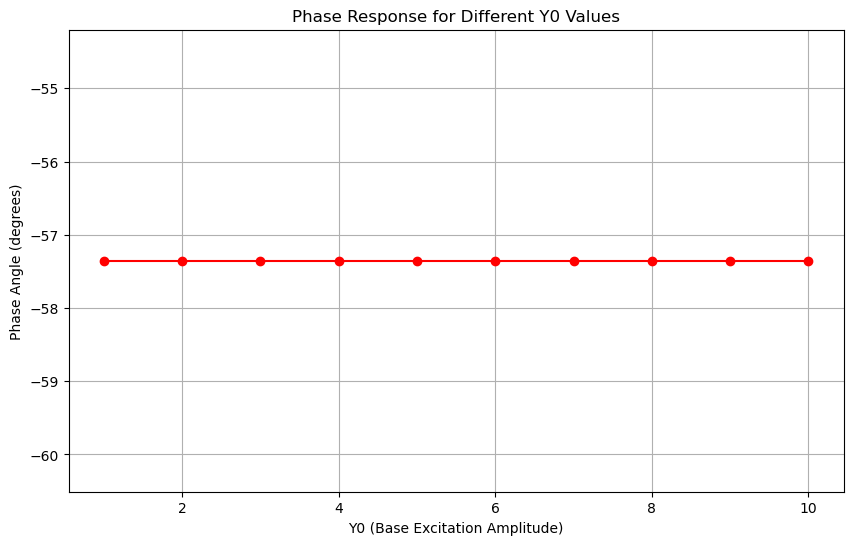
\includegraphics[width=0.8\textwidth]{phase_resp.png} 
    \caption{Phase Response for different Y0 values}
    \label{fig:system}
\end{figure}
{\vspace{10pt}}
Discussion ...
{\vspace{10pt}}

    
\end{document}
